In Hops for reasons that I have outlined in previous chapters we
persist all the metadata in our persistent storage solution. MySQL
Cluster is a relational distributed database, so data are stored into
tables with very specific properties. Since version 7.3.1, MySQL
Cluster supports foreign key constraints. Foreign keys is a powerful
feature of relational databases that guarantee some kind of
consistency between two tables. One important aspect of foreign keys
is that they map relationships of the ``real-world'' into
relationships in the database.

The database schema of Hops consists of 95 tables, 64 out of them are
used by Hops-YARN. The information they store span from incoming RPCs
to scheduler state and nodes' statuses. We make heavy use of foreign
key constraints, mainly the \texttt{ON DELETE} referential action, to
ensure integrity when a row from a parent table is deleted. Although
the database schema of Hops-YARN is too big to fit in
a single page, Figure \ref{fig:impl_fk_yarn_schema}, the number of
foreign key relationships -- they are illustrated with a solid line --
is clear. There our two reasons why we actually have relationships
between tables. The first one is because there is indeed semantically a
relationship between the tables. For example in Figure
\ref{fig:impl_fk_yarn_rmnode}, the table \texttt{yarn\_rmnode} is used by
the RM to store information regarding the available nodes in
the cluster. Table \texttt{yarn\_containerstatus} on the same figure
stores some status information for the containers that have been
launched. Obviously there is a relationship between the containers and
the nodes of a Hadoop cluster. A container cannot be launched in a
node that has not been registered with the RM yet. Similarly,
a container should not exists in the database if the node row has been
deleted. The second usage of foreign keys is to group together tables,
such as the tables in Figure \ref{fig:impl_fk_yarn_rpc}. These tables
persist the heartbeats sent by the AMs and NMs. For a reason that will
be explained in Section \ref{ssec:impl_fk_alloc_resp}, the information that a
single heartbeat carries had to be partitioned and stored in multiple
tables. Again, we do not want orphan entries and we avoid this by the
\texttt{ON DELETE} action.

Foreign keys in relational databases is a great feature. They do not
come without a cost though. For bulk and frequent operations they kill
performance. In our case that we want to scale to 10k nodes in a
cluster it means that we have to remove these constraints and replace
them with some logic in the program that will cascade the deletion to
children tables. It is very important that this logic will make
\textbf{primary key} operations for two reasons. The first reason, which
applies to all relational databases, is that primary keys are indexed,
so you avoid making full table scan. The indexes usually are
implemented with a \texttt{B-tree} and/or hash table data structure which allows
operations in logarithmic or constant time depending on the query. The second reason, which applies
specifically to NDB, is that primary keys are also partition keys, if
no partition keys are defined explicitly. A
partition key defines how data will be distributed across Data Nodes
in the MySQL Cluster. Executing statements based on the primary key,
alleviates the round-trip time between the Data Nodes, since NDB will
know exactly in which machine the row you are looking for is
stored. In non primary key operations, NDB might have to lookup in all
Data Nodes to execute the statement.

Although the main reason we use foreign keys is to get the
automatic cascading in the deletion of a row, this has a side effect to
insertion operations also. A row in a child table cannot be inserted
in the database before its parent, otherwise the RDBMS will complain
about missing foreign key. To solve it we have to insert the parent
row, then \emph{flush} the buffer and then insert the child row which
imposes an order and cancels out any parallelism. In the rest of this section I will describe how I achieved
this for every parent table that had foreign keys to other children tables.

\begin{figure}
\centering
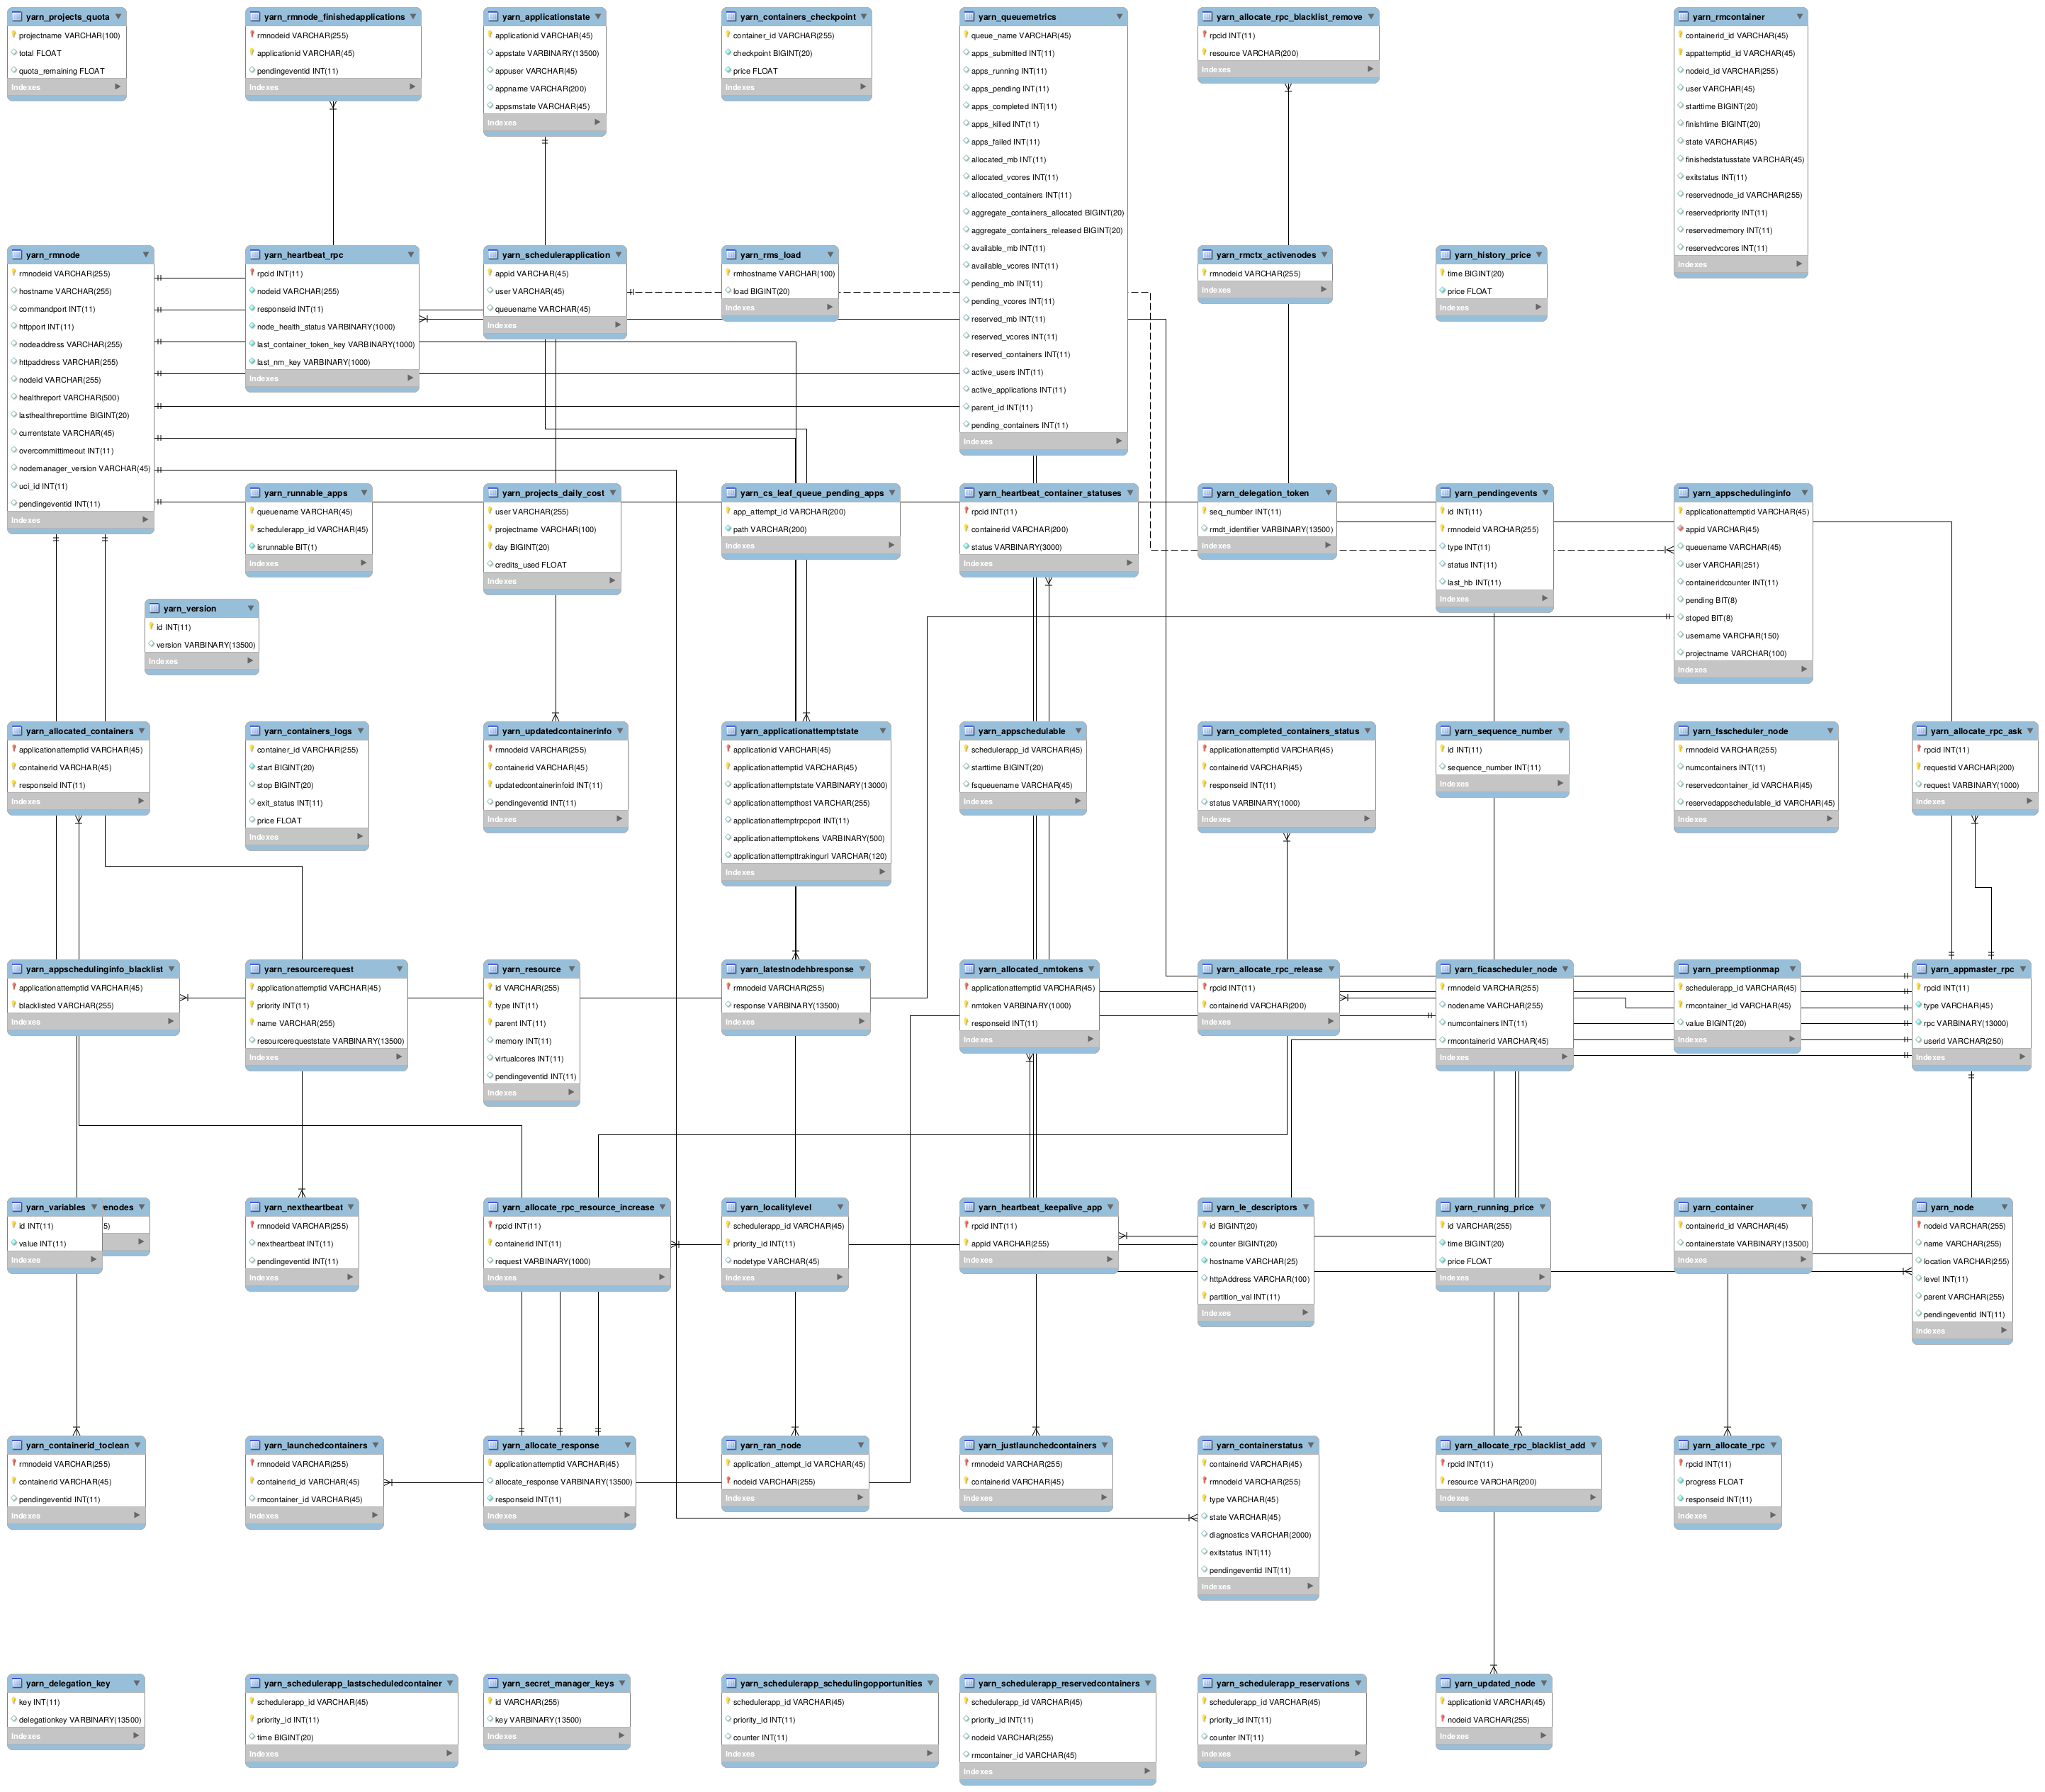
\includegraphics[scale=0.2,angle=90]{resources/images/Implementation/hops_yarn_ndb_schema_full.png}
\caption{Hops-YARN database schema}
\label{fig:impl_fk_yarn_schema}
\end{figure}

\begin{figure}
\centering
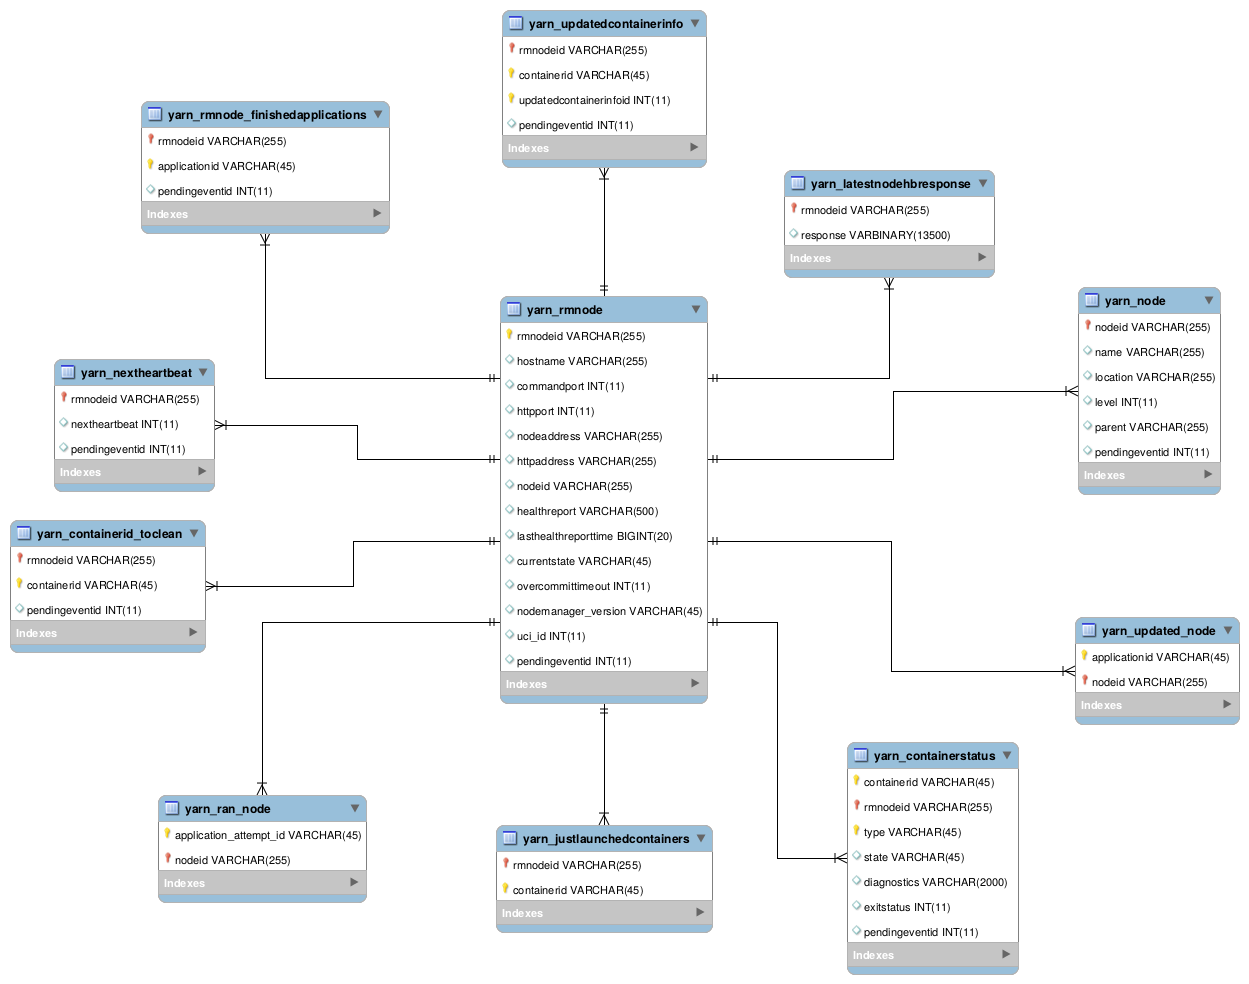
\includegraphics[scale=0.4]{resources/images/Implementation/hops_yarn_ndb_schema_rmnode.png}
\caption{A node in the cluster from the scheduler's perspective}
\label{fig:impl_fk_yarn_rmnode}
\end{figure}

\begin{figure}
\centering
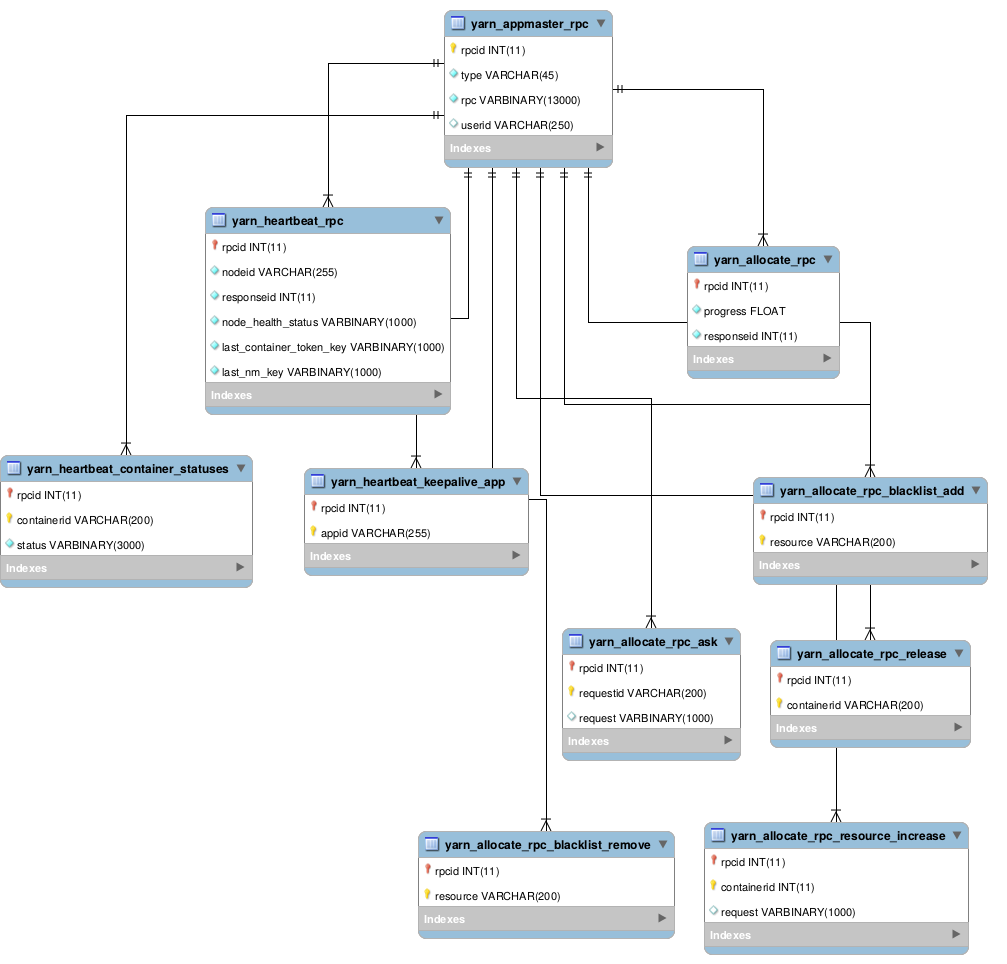
\includegraphics[scale=0.4]{resources/images/Implementation/hops_yarn_ndb_schema_rpc.png}
\caption{Database tables to store incoming RPCs}
\label{fig:impl_fk_yarn_rpc}
\end{figure}

\subsection{yarn\_rmnode}
\label{ssec:impl_fk_rmnode}
NodeManager is the process that runs on every physical node on a
Hadoop cluster. The scheduler keeps information for every NM
represented by the \texttt{RMNode} class. The information this
class holds is persisted in the \texttt{yarn\_rmnode} table, Figure
\ref{fig:impl_fk_yarn_rmnode}. This table is parent table to
numerous other tables such as \texttt{yarn\_node} which holds
information about the name of the node, its location etc. Another
table is
\texttt{yarn\_latestnodehbresponse} which holds the last response sent
by the RM to that NM. In total there are 10 tables having foreign key
constraints to \texttt{yarn\_rmnode}. Ideally we would like to replace
them with a logic that performs deletions with primary key
operations. The problem in that case is that the children tables are
diverse and have multi-column primary keys, so keeping in memory all
the primary keys would not be efficient. Especially when the deletion
operation of an RMNode would not happen very frequently, only in the case
of a dead node. Moreover, in later versions of YARN, RMNodes are never
removed from RM's state, just having their status changed.

With all these in mind we decided to remove the foreign key
constraints from the children without doing primary key
operations. In the client library we have implemented for NDB,
I wrote logic that whenever an RMNode row would be deleted, this
deletion would be cascaded to the rest of the tables. Children tables
have the \texttt{rmnodeid} either as part of their primary key or indexed, so we
avoid a full table scan. The implementation was very straightforward,
when the remove method in the client library is called for an RMNode,
I select all the rows from the corresponding tables filtered by the
\texttt{rmnodeid} and finally remove them. Considering that this
operation would occur rarely and in later versions never, that was a
fine solution trading performance with memory usage.

\subsection{yarn\_allocate\_response}
\label{ssec:impl_fk_alloc_resp}
Next in the list with tables that are referenced with foreign keys is
\texttt{yarn\_allocate\_response}. It holds the response sent by the
RM to an allocate request by an AM. This is the case where we had to
partition the data persisted. MySQL Cluster has a limit to the size of
a single row. That limit is 14000 bytes \cite{ndb_row_limit} and in
some cases the data that are to be persisted exceeds it. So the
allocation response is partitioned to
\texttt{yarn\_allocated\_containers} and
\texttt{yarn\_completed\_containers\_status}, both having foreign keys
to \texttt{yarn\_allocate\_response}. Since the deletion operation of
an allocate response would happen very often, primary key operation
was the only way to achieve high performance. Both tables have a
multi-column primary key with the \texttt{applicationattemptid}, the
\texttt{containerid} and the \texttt{responseid}. An allocate response
is removed from the database when $(1)$ a new response for that
application is created, $(2)$ the ApplicationMaster unregisters with
the RM. The first case will be examined in Section
\ref{sec:gc_service}. When an application unregisters I get all the
container IDs that the application was using from the RM in-memory
state and the response ID,
then I build the primary keys and issue primary key deletion
operations for those three tables in parallel.

\subsection{yarn\_ficascheduler\_node}
\label{ssec:impl_fk_fica_node}
The scheduler, and specifically Fifo and Capacity, holds information for the nodes in the cluster in its
own data structure identified by the class \texttt{FiCaSchedulerNode}. This
class is persisted in NDB in the table
\texttt{yarn\_ficascheduler\_node} which is parent for the table
\texttt{yarn\_launchedcontainers}. The later keeps a map of the
container IDs that are launched to a scheduler node. Its primary key
consists of the \texttt{nodeid} (FiCaNode) and the
\texttt{containerid}. The delete method on
\texttt{yarn\_ficascheduler\_node} Data Access Object is called when a
node is deleted from the scheduler's view. At that point the node
representation already holds the IDs of the containers that were
running on that node. Similarly, I construct the primary keys for the
child table for every \texttt{containerid} and issue the deletion operation for both
\texttt{yarn\_ficascheduler\_node} row and
\texttt{yarn\_launchedcontainers} rows.

\subsection{yarn\_applicationstate}
\label{ssec:impl_fk_appstate}
Hops-YARN persists in the database back-end the state of every
application scheduled. This state includes information such as the
name and the user of the application, the \emph{Application submission
  context}, diagnostics etc. Since applications and specifically AMs
can fail, YARN also tracks the attempts an application made to be scheduled.
If the AM fails, then YARN creates a new application attempt
for that application and spawns the new AM. The state of the
application is stored in \texttt{yarn\_applicationstate} table in the
database and every attempt for that application in
\texttt{yarn\_applicationattemptstate}. Application attempt
semantically has a relationship with the application and in the
relational world is expressed with a foreign key constraint
between \texttt{yarn\_applicationstate} (parent) and
\texttt{yarn\_applicationattemptstate} (child). When an application
is completed it is removed from the state of the scheduler and all
its attempts. Reconstructing the primary key for the attempts table
\texttt{<applicationid, applicationattemptid>} is trivial since the
application object holds the IDs of its attempts.

\subsection{yarn\_appschedulinginfo}
\label{ssec:impl_fk_appschedulinginfo}
An application from the scheduler's (Fifo, Capacity) point of view is
represented by the class \texttt{FiCaSchedulerApp}. This class
contains data structures that should be persisted such as resource
requests, the application attempt, any blacklisted resources etc. All
this information is stored in \texttt{yarn\_appschedulinginfo} table
which is parent to \texttt{yarn\_appschedulinginfo\_blacklist}
containing blacklisted resources for a specific application
attempt. In order to efficiently remove blacklisted resources when an
\texttt{yarn\_appschedulinginfo} row is removed, I have to construct
the primary key of \texttt{yarn\_appschedulinginfo\_blacklist} which
consists of the application attempt ID and the ID of the blacklisted
resource and then execute the delete operations.

\subsection{yarn\_schedulerapplication}
\label{ssec:impl_fk_schedulerapp}
\texttt{SchedulerApplication} class is the base class for
\texttt{FiCaSchedulerApp} that we have examined previously. This
naturally translates into a foreign key constraint between
\texttt{yarn\_appschedulinginfo} -- child, and \\
\texttt{yarn\_schedulerapplication} -- parent. In this case we have
three tables chained together with foreign keys. A deletion in table 
\texttt{yarn\_schedulerapplication}, will trigger a deletion in
\texttt{yarn\_appschedulinginfo} which in turn trigger a deletion in
\texttt{yarn\_appschedulinginfo\_blacklist}. This greatly deteriorates
the performance both for insert and delete operations. The foreign
keys dictate a very strict order on the insertion of rows in these
tables. If these statements are executed in parallel then there is no
guarantee about the order and an error might occur compromising the data. That
limitation forces us to excessively flush the buffer of the
transaction manager introducing network latency.

\subsection{yarn\_appmaster\_rpc}
\label{ssec:impl_fk_appmaster_rpc}
Finally, the last table that other tables had references to, was
\texttt{yarn\_appmaster\_rpc}. The database schema is illustrated in
Figure \ref{fig:impl_fk_yarn_rpc}. These tables are used to persist
incoming RPCs so in a crash scenario, the RM would recover and replay
them. At the time of replacing the foreign key relationships with
primary key operations we have decided to leave this set of tables as
it is. Later we saw that this setup was greatly affecting the
performance and the mechanism described in Section
\ref{sec:gc_service} came in place.

Having all, or most of, the foreign key constraints replaced by
primary key operations improved performance and made the database
schema more flexible. Performance was increased for two
reasons. Without any constraint we are able to remove the
\texttt{flush} operations from transactions. In some cases we do need
to maintain an order in our operations but that is limited. Removing
flushes allowed for increased \textbf{parallelism} in database operations while decreased the
network \textbf{latency} that we were paying for every flush
operation. In most of the cases, building the multi-column primary key
was an easy task but it was a great opportunity to get familiar with
YARN and NDB and a good warm-up for the changes to come.
